% Chapter Template

\chapter{Design of Data-Acquisition System with Cluster-Finding Trigger} % Main chapter title

\label{Chapter4} % Change X to a consecutive number; for referencing this chapter elsewhere, use \ref{ChapterX}

% outline
%----------------------------------------------------------------------------
% 4-1 : Overview of the KOTO DAQ 
% 4-2 : 
% 4-3 : 
% 4-4 : 

A valid physics event, which in general represents a $K_L^0$ decay, contains the hit variables from the entire detector. Those variables are obtained by analyzing the pulses from nearly 4000 channels. Because the $K_L^0$ decay time is not controllable, a methodology needs to be established to record the pulses at the appropriate moment.


the data-acquisition (DAQ) system is supposed to collect the signals from all channels at the suitable moment. Furthermore, due to the hardware limitation, the three-level trigger system is designed to suppress the background-like events and maximally collect the signals under the high-flux beam. 

The KOTO DAQ system had been elaborately upgraded since 2017 to improve the collection efficiency, the rate control, and the flexibility to various physics topics. The overall architecture is explained in this chapter. 

%----------------------------------------------------------------------------------------
%	SECTION 1: Overview of the KOTO DAQ
%----------------------------------------------------------------------------------------

\section{Overview of the KOTO Data-Acquisition System}
The fundamental concept of the KOTO DAQ system is the pipeline readout, as shown in Figure~\ref{fig:pipeline}. The signals from nearly 4000 channels are continuously digitized by the customized flush-analog-to-digital converter (FADC) at either 125 MHz or 500 MHz, and recorded in the memory. The size of the memory for the input data stream corresponds to 5.2~$\SI{}{\mu}$s, known as the pipeline depth, and  



%The memory in the Field Programmable Gate Array (FPGA) on each FADC board keeps updating the input signal within the past 5.2~$\SI{}{\mu}$s, known as the pipeline depth. During this period, the advantageous features are extracted out from the inputs and delivered to the trigger core for further analysis.  


\begin{figure}[h]
\begin{center}
\captionsetup{width=.99\linewidth}
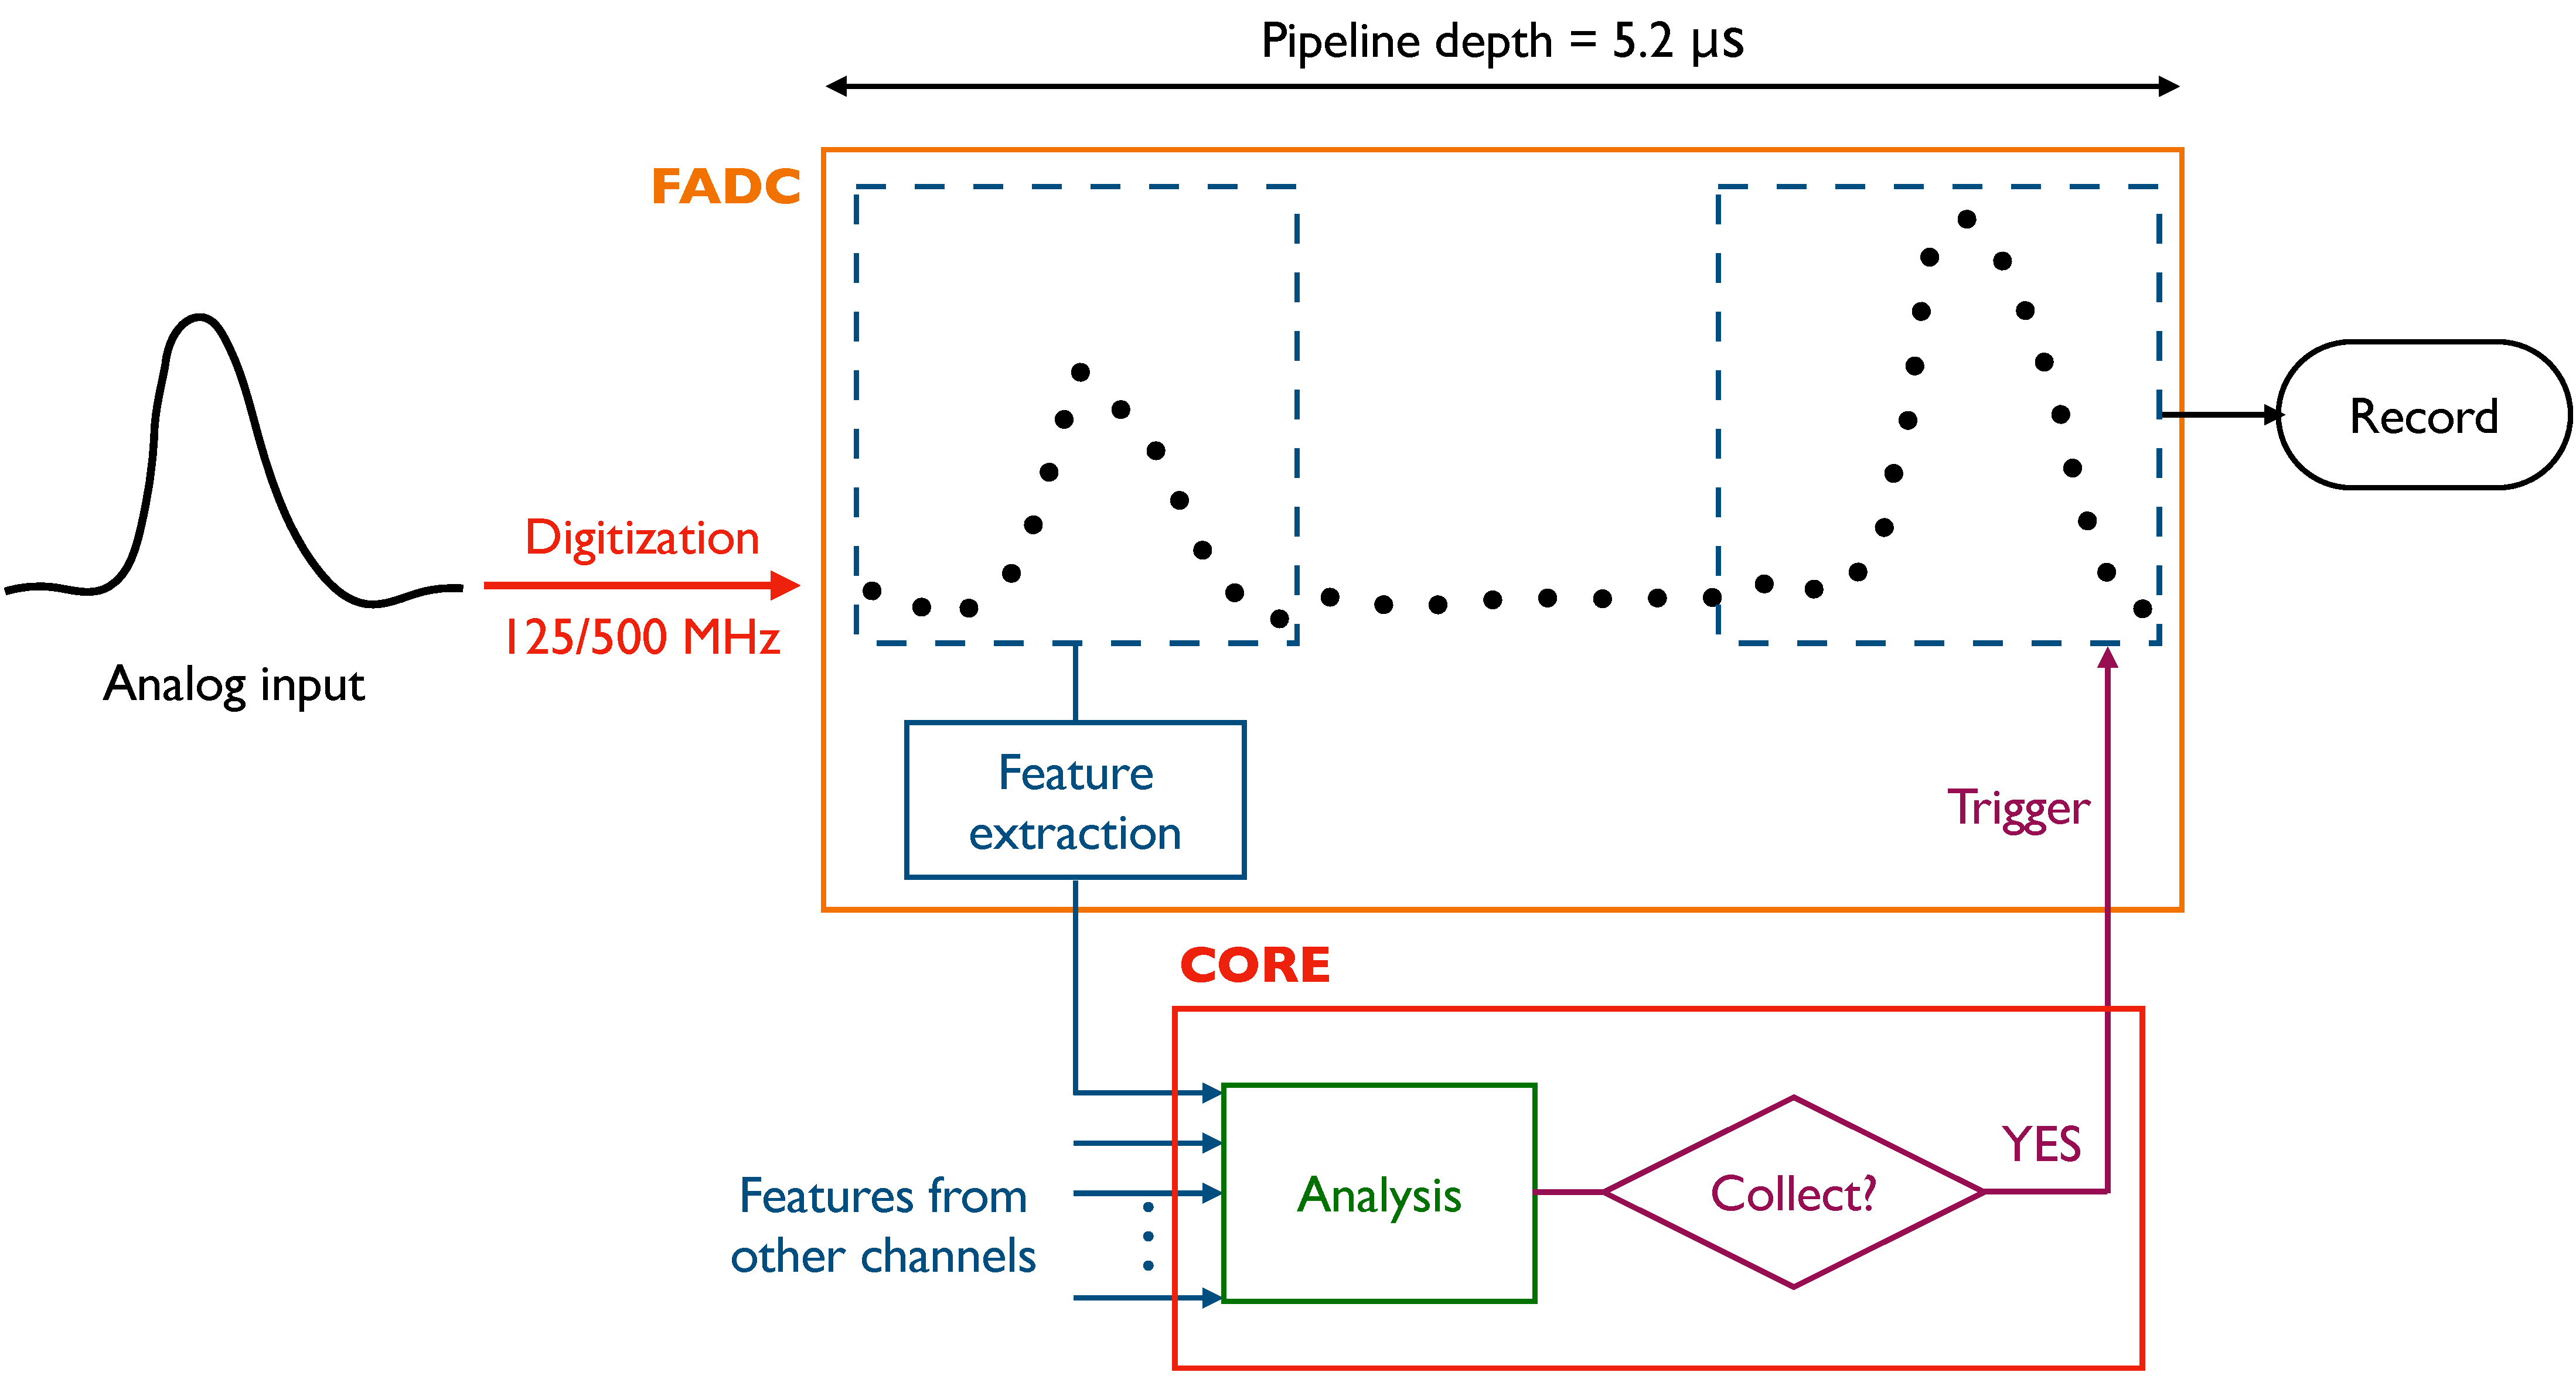
\includegraphics[width=0.99\textwidth]{Figures/Chapter4/pipeline.pdf}
\caption{Fundamental concept of the KOTO trigger. }
\label{fig:pipeline}
\end{center}
\end{figure}


% side caption
%\begin{figure}[h]
% \begin{minipage}[c]{0.5\textwidth}
%    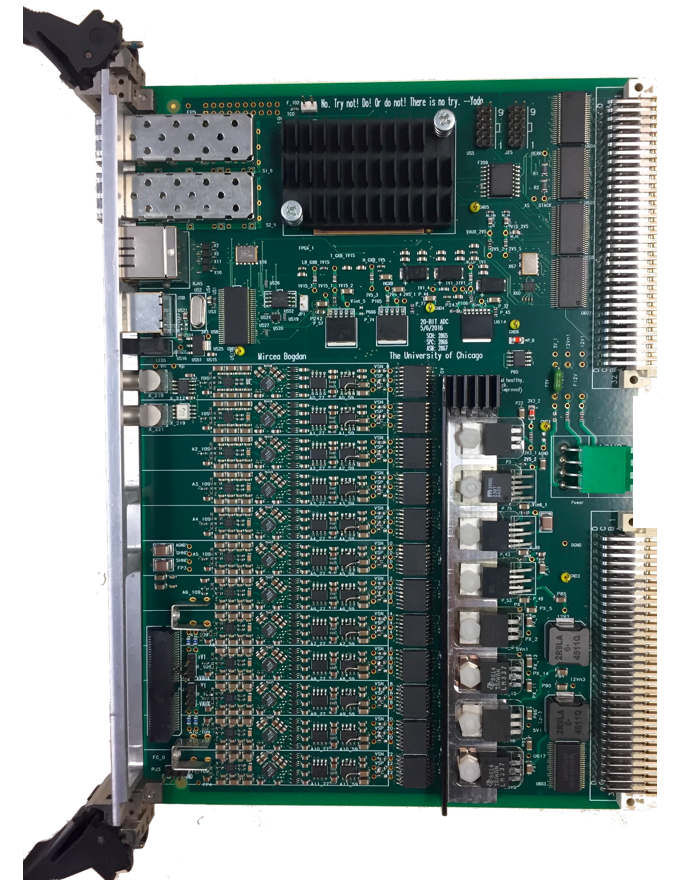
\includegraphics[width=\textwidth]{Figures/Chapter4/ADC.png}
%  \end{minipage}\hfill
%  \begin{minipage}[c]{0.5\textwidth}
%    \captionsetup{width=.99\linewidth}
%    \vspace*{\fill}
%    \caption{
%       A picture of 125-MHz ADC.
%    } \label{fig:ADC_pic}
%  \end{minipage}
%\end{figure}


\section{test}


\parencite{125MHz_ADC}

\begin{figure}[h]
\begin{center}
\captionsetup{width=.99\linewidth}
\includegraphics[width=0.99\textwidth]{Figures/Chapter4/ADC_picture.pdf}
\caption{A picture of a 125-MHz FADC (left) and a 500-MHz FADC (right) board manufactured by University of Chicago  (Figure courtesy of \parencite{mircea}). A 125-MHz (500-MHz) consists of 16 (4) analog inputs, two RJ-45 connectors for LVDS transmission, two optical fiber connectors, and an FPGA of Altera.}
\label{fig:ADC_picture}
\end{center}
\end{figure}


